\let\negmedspace\undefined
\let\negthickspace\undefined
\documentclass[journal]{IEEEtran}
\usepackage[a5paper, margin=9mm, onecolumn]{geometry}
\usepackage{lmodern} 
\usepackage{tfrupee} 

\setlength{\headheight}{1cm} 
\setlength{\headsep}{0mm}     

\usepackage{gvv-book}
\usepackage{gvv}
\usepackage{cite}
\usepackage{amsmath,amssymb,amsfonts,amsthm}
\usepackage{algorithmic}
\usepackage{graphicx}
\usepackage{textcomp}
\usepackage{xcolor}
\usepackage{txfonts}
\usepackage{listings}
\usepackage{enumitem}
\usepackage{mathtools}
\usepackage{gensymb}
\usepackage{comment}
\usepackage{multicol}
\usepackage[breaklinks=true]{hyperref}
\usepackage{tkz-euclide} 
\usepackage{listing}

\graphicspath{ {./figs/} }

\begin{document}


\title{
ASSIGNMENT 5: GATE 2023\\
IN:INSTRUMENTATION ENGINEERING}
\author{AI25BTECH11013-Gautham Pocha}
\maketitle
\renewcommand{\thefigure}{\theenumi}
\renewcommand{\thetable}{\theenumi}

\begin{enumerate}
    \item The village was nestled in a green spot, \_\_\_\_\_ the ocean and the hills.
    
    \begin{enumerate}
        \item through
        \item in
        \item at
        \item between
    \end{enumerate}
    \hfill(GATE IN 2023)

    \item Disagree : Protest : : Agree : \_\_\_\_\_ (By word meaning)
    
    \begin{enumerate}
        \item Refuse
        \item Pretext
        \item Recommend
        \item Refute
    \end{enumerate}
    \hfill(GATE IN 2023)

    \item A 'frabjous' number is defined as a 3 digit number with all digits odd, and no two adjacent digits being the same. For example, 137 is a frabjous number, while 133 is not. How many such frabjous numbers exist?
    
    \begin{enumerate}
        \item 125
        \item 720
        \item 60
        \item 80
    \end{enumerate}
    \hfill(GATE IN 2023)

    \item Which one among the following statements must be TRUE about the mean and the median of the scores of all candidates appearing for GATE 2023?
    
    \begin{enumerate}
        \item The median is at least as large as the mean.
        \item The mean is at least as large as the median.
        \item At most half the candidates have a score that is larger than the median.
        \item At most half the candidates have a score that is larger than the mean.
    \end{enumerate}
    \hfill(GATE IN 2023)

    \item In the given diagram, ovals are marked at different heights ($h$) of a hill. Which one of the following options P, Q, R, and S depicts the top view of the hill?
    \begin{figure}[H]
    \centering
      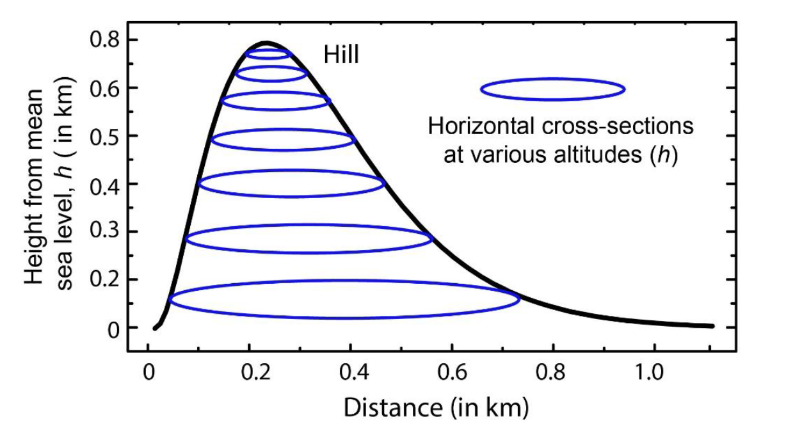
\includegraphics[width=0.6\textwidth]{1.png} 
      \caption{}
    \label{fig:fig1} 
    \end{figure}
    \begin{multicols}{2}
    \begin{figure}[H]
      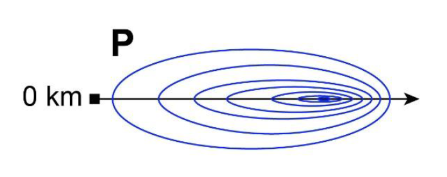
\includegraphics[width=0.3\textwidth]{2.png} 
      \caption{}
    \label{fig:fig2} 
\end{figure}
\begin{figure}[H]
      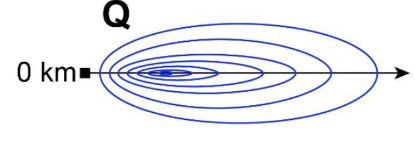
\includegraphics[width=0.3\textwidth]{3.png} 
      \caption{}
    \label{fig:fig3} 
\end{figure}
\begin{figure}[H]
      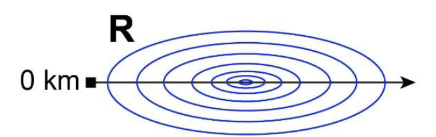
\includegraphics[width=0.3\textwidth]{4.png} 
      \caption{}
    \label{fig:fig4} 
\end{figure}
\begin{figure}[H]
      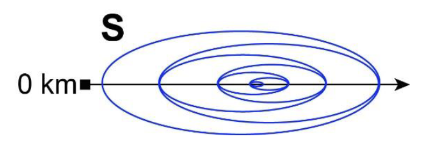
\includegraphics[width=0.3\textwidth]{5.png} 
      \caption{}
    \label{fig:fig5} 
\end{figure}
\end{multicols}
    \begin{enumerate}
        \item P
        \item Q
        \item R
        \item S
    \end{enumerate}
    \hfill(GATE IN 2023)

    \item Residency is a famous housing complex with many well-established individuals among its residents. A recent survey conducted among the residents of the complex revealed that all of those residents who are well established in their respective fields happen to be academicians. The survey also revealed that most of these academicians are authors of some best-selling books. Based only on the information provided above, which one of the following statements can be logically inferred with certainty?
    
    \begin{enumerate}
        \item Some residents of the complex who are well established in their fields are also authors of some best-selling books.
        \item All academicians residing in the complex are well established in their fields.
        \item Some authors of best-selling books are residents of the complex who are well established in their fields.
        \item Some academicians residing in the complex are well established in their fields.
    \end{enumerate}
    \hfill(GATE IN 2023)

    \item Ankita has to climb 5 stairs starting at the ground, while respecting the following rules: 
    \begin{enumerate}
        \item At any stage, Ankita can move either one or two stairs up.
        \item At any stage, Ankita cannot move to a lower step.
    \end{enumerate}
    Let $F(N)$ denote the number of possible ways in which Ankita can reach the $N$th stair. For example, $F(1) = 1$, $F(2) = 2$, $F(3) = 3$. The value of $F(5)$ is \_\_\_\_\_.
    
    \begin{enumerate}
        \item 8
        \item 7
        \item 6
        \item 5
    \end{enumerate}
    \hfill(GATE IN 2023)

    \item The information contained in DNA is used to synthesize proteins that are necessary for the functioning of life. DNA is composed of four nucleotides: Adenine (A), Thymine (T), Cytosine (C), and Guanine (G). The information contained in DNA can then be thought of as a sequence of these four nucleotides: A, T, C, and G. DNA has coding and non-coding regions. Coding regions—where the sequence of these nucleotides are read in groups of three to produce individual amino acids—constitute only about 2\% of human DNA. For example, the triplet of nucleotides CCG codes for the amino acid glycine, while the triplet GGA codes for the amino acid proline. Multiple amino acids are then assembled to form a protein. Based only on the information provided above, which of the following statements can be logically inferred with certainty?
    \begin{enumerate}
        \item[(i)] The majority of human DNA has no role in the synthesis of proteins.
        \item[(ii)] The function of about 98\% of human DNA is not understood.
    \end{enumerate}
    
    \begin{enumerate}
        \item only (i)
        \item only (ii)
        \item both (i) and (ii)
        \item neither (i) nor (ii)
    \end{enumerate}
    \hfill(GATE IN 2023)

    \item Which one of the given figures P, Q, R and S represents the graph of the following function?
    $$f(x) = ||x+2| - |x-1||$$
        \begin{multicols}{2}
    \begin{figure}[H]
      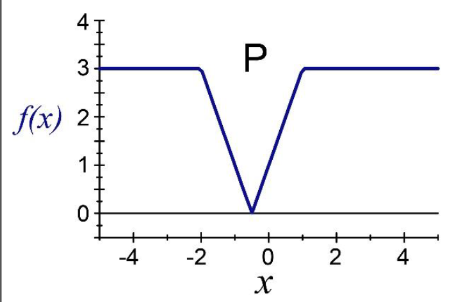
\includegraphics[width=0.3\textwidth]{6.png} 
      \caption{}
    \label{fig:fig6} 
\end{figure}
\begin{figure}[H]
      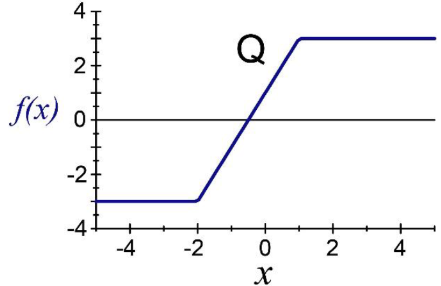
\includegraphics[width=0.3\textwidth]{7.png} 
      \caption{}
    \label{fig:fig7} 
\end{figure}
\begin{figure}[H]
      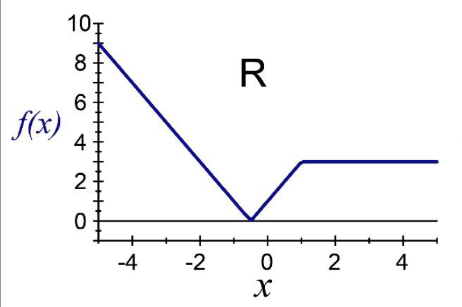
\includegraphics[width=0.3\textwidth]{8.png} 
      \caption{}
    \label{fig:fig8} 
\end{figure}
\begin{figure}[H]
      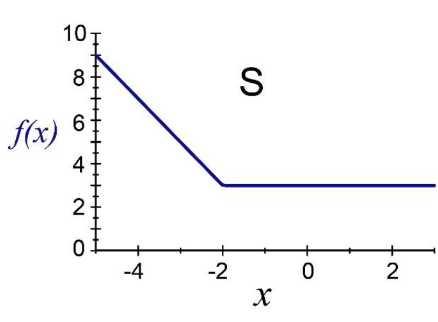
\includegraphics[width=0.3\textwidth]{9.png} 
      \caption{}
    \label{fig:fig9} 
\end{figure}
\end{multicols}
    
    \begin{enumerate}
        \item P
        \item Q
        \item R
        \item S
    \end{enumerate}
    \hfill(GATE IN 2023)

    \item An opaque cylinder (shown below) is suspended in the path of a parallel beam of light, such that its shadow is cast on a screen oriented perpendicular to the direction of the light beam. The cylinder can be reoriented in any direction within the light beam. Under these conditions, which one of the shadows P, Q, R, and S is NOT possible?
        \begin{multicols}{2}
        \begin{figure}[H]
    \centering
      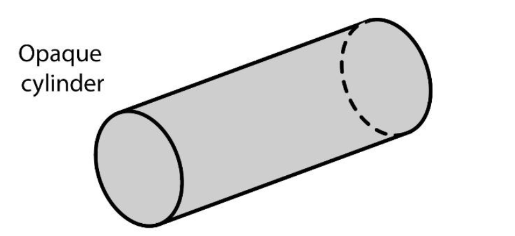
\includegraphics[width=0.6\textwidth]{10.png} 
      \caption{}
    \label{fig:fig10} 
\end{figure}
    \begin{figure}[H]
      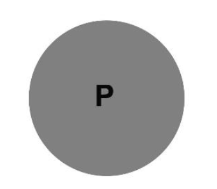
\includegraphics[width=0.3\textwidth]{11.png} 
      \caption{}
    \label{fig:fig11} 
\end{figure}
\begin{figure}[H]
      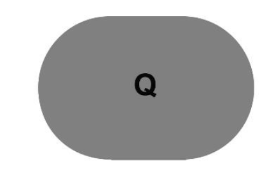
\includegraphics[width=0.3\textwidth]{12.png} 
      \caption{}
    \label{fig:fig12} 
\end{figure}
\begin{figure}[H]
      
\includegraphics[width=0.3\textwidth]{13.png} 
      \caption{}
    \label{fig:fig13} 
\end{figure}
\begin{figure}[H]
      
\includegraphics[width=0.3\textwidth]{14.png} 
      \caption{}
    \label{fig:fig14} 
\end{figure}
\end{multicols}
    \begin{enumerate}
        \item P
        \item Q
        \item R
        \item S
    \end{enumerate}
    \hfill(GATE IN 2023)

    \item Choose solution set $S$ corresponding to the systems of two equations
    \begin{align*}
    x - 2y + z &= 0 \\
    x - z &= 0
    \end{align*}
    Note: $\mathbb{R}$ denotes the set of real numbers
    
    \begin{enumerate}
        \item $S = \left\{ \alpha \myvec{ 1 \\ 1 \\ 1 } \middle| \alpha \in \mathbb{R} \right\}$
        \item $S = \left\{ \alpha \myvec{ 1 \\ 1 \\ 1 } + \beta \myvec{ 1 \\ 0 \\ 1 } \middle| \alpha, \beta \in \mathbb{R} \right\}$
        \item $S = \left\{ \alpha \myvec{ 1 \\ 1 \\ 1 } + \beta \myvec{ 2 \\ 1 \\ 2 } \middle| \alpha, \beta \in \mathbb{R} \right\}$
        \item $S = \left\{ \alpha \myvec{ 1 \\ 0 \\ 1 } \middle| \alpha \in \mathbb{R} \right\}$
    \end{enumerate}
    \hfill(GATE IN 2023)

    \item Inductance of a coil is measured as 10 mH, using an LCR meter, when no other objects are present near the coil. The LCR meter uses a sinusoidal excitation at 10 kHz. If a pure copper sheet is brought near the coil, the same LCR meter will read\_\_\_\_\_.
    
    \begin{enumerate}
        \item less than 10 mH
        \item 10 mH
        \item more than 10 mH
        \item less than 10 mH initially and then stabilizes to more than 10 mH
    \end{enumerate}
    \hfill(GATE IN 2023)

    \item Which of the following flow meters offers the lowest resistance to the flow?
    
    \begin{enumerate}
        \item Turbine flow meter
        \item Orifice flow meter
        \item Venturi meter
        \item Electromagnetic flow meter
    \end{enumerate}
    \hfill(GATE IN 2023)

    \item Pair the quantities (p) to (s) with the measuring devices (i) to (iv).
    
\begin{table}[H]
\begin{tabular}{c c}
i.Linear Variable Differential Transformer (LVDT)& p. Torque \\
ii. Thermistor & q. Pressure \\
iii. Strain gauge & r.Linear position  \\
iv.Diaphragm & s.Temperature \\
\end{tabular}
\caption{}
\label{tab:matching 1}
\end{table}
    \begin{enumerate}
        \item (i) - (r), (ii) - (s), (iii) - (q), (iv) - (p)
        \item (i) - (p), (ii) - (s), (iii) - (r), (iv) - (q)
        \item (i) - (r), (ii) - (s), (iii) - (p), (iv) - (q)
        \item (i) - (q), (ii) - (s), (iii) - (p), (iv) - (r)
    \end{enumerate}
    \hfill(GATE IN 2023)

    \item Capacitance 'C' of a parallel plate structure is calculated as 20 pF using $C = \varepsilon_0 \varepsilon_r A / d$, where $\varepsilon_0$ is the permittivity of free space, $\varepsilon_r$ is the relative permittivity of the dielectric, $A$ is the overlapping area of the electrodes and $d$ is the distance between them. The value of $C$ is then measured using an LCR meter. If the meter is assumed to be ideal and it introduces no error due to cable capacitance, which one of the following readings is likely to be correct?
    
    \begin{enumerate}
        \item 20.5 pF
        \item 20 pF
        \item 19.5 pF
        \item 10 pF
    \end{enumerate}
    \hfill(GATE IN 2023)

    \item The table shows the present state $Q(t)$, next state $Q(t+1)$, and the control input in a flip-flop. Identify the flip-flop.
    \begin{table}[H]
    \begin{tabular}{|c|c|c|}
    \hline
    $Q(t)$ & $Q(t+1)$ & Input \\
    \hline
    0 & 0 & 0 \\
    0 & 1 & 1 \\
    1 & 0 & 1 \\
    1 & 1 & 0 \\
    \hline
    \end{tabular}
    \caption{}
    \label{tab:table1}
    \end{table}
    
    \begin{enumerate}
        \item T flip-flop
        \item D flip-flop
        \item SR flip-flop
        \item JK flip-flop
    \end{enumerate}
    \hfill(GATE IN 2023)

    \item Match the Exclusive-OR (XOR) operations (i) to (iv) with the results (p) to (s), where $X$ is a Boolean input.
    \begin{table}[H]
\begin{tabular}{c c}
i.$X \oplus X$& p. 1 \\
ii. $X \oplus \overline{X}$ & q. 0 \\
iii.$X \oplus 0$ & r.$X$  \\
iv. $X \oplus 1$& s.$\overline{X}$\\
\end{tabular}
\caption{}
\label{tab:matching 2}
\end{table}
    
    \begin{enumerate}
        \item (i) - (q), (ii) - (r), (iii) - (s), (iv) - (p)
        \item (i) - (q), (ii) - (r), (iii) - (p), (iv) - (s)
        \item (i) - (p), (ii) - (s), (iii) - (q), (iv) - (r)
        \item (i) - (q), (ii) - (p), (iii) - (s), (iv) - (r)
    \end{enumerate}
    \hfill(GATE IN 2023)

    \item A light emitting diode (LED) emits light when it is \_\_\_\_\_biased. A photodiode provides maximum sensitivity to light when it is\_\_\_\_\_biased.
    
    \begin{enumerate}
        \item forward, forward
        \item forward, reverse
        \item reverse, reverse
        \item reverse, forward
    \end{enumerate}
    \hfill(GATE IN 2023)

    \item $F(z) = \frac{1}{1-z}$ when expanded as a power series around $z = 2$, would result in $F(z) = \sum_{k=0}^{\infty} \alpha_k (z-2)^k$, with the region of convergence (ROC) $|z-2| < 1$. The coefficients $\alpha_k$, $k \geq 0$, are given by the expression\_\_\_\_\_.
    
    \begin{enumerate}
        \item $(-1)^k$
        \item $(-1)^{k+1}$
        \item $\frac{1}{2^k}$
        \item $\frac{(-1)^{k+1}}{2^k}$
    \end{enumerate}
    \hfill(GATE IN 2023)

    \item The solution $x(t)$, $t \geq 0$, to the differential equation $\ddot{x} = -k\dot{x}$, $k > 0$ with initial conditions $x(0) = 1$ and $\dot{x}(0) = 0$ is
    
    \begin{enumerate}
        \item $x(t) = 2e^{-kt} + 2kt - 1$
        \item $x(t) = 2e^{-kt} - 1$
        \item $x(t) = 1$
        \item $x(t) = 2e^{-kt} - kt - 1$
    \end{enumerate}
    \hfill(GATE IN 2023)

    \item A system has the transfer-function $\frac{Y(s)}{X(s)} = \frac{s-\pi}{s+\pi}$. Let $u(t)$ be the unit-step function. The input $x(t)$ that results in a steady-state output $y(t) = \sin \pi t$ is \_\_\_\_\_.
    
    \begin{enumerate}
        \item $x(t) = \sin(\pi t) u(t)$
        \item $x(t) = \sin\left(\pi t + \frac{\pi}{2}\right) u(t)$
        \item $x(t) = \sin\left(\pi t - \frac{\pi}{2}\right) u(t)$
        \item $x(t) = \cos\left(\pi t + \frac{\pi}{4}\right) u(t)$
    \end{enumerate}
    \hfill(GATE IN 2023)

    \item Choose the fastest logic family among the following:
    
    \begin{enumerate}
        \item Transistor-Transistor Logic
        \item Emitter-Coupled Logic
        \item CMOS Logic
        \item Resistor-Transistor Logic
    \end{enumerate}
    \hfill(GATE IN 2023)

    \item What is $\lim_{x \to 0} f(x)$, where $f(x) = x \sin \frac{1}{x}$?
    
    \begin{enumerate}
        \item 0
        \item 1
        \item $\infty$
        \item Limit does not exist
    \end{enumerate}
    \hfill(GATE IN 2023)

    \item The number of zeros of the polynomial $P(s) = s^3 + 2s^2 + 5s + 80$ in the right-half plane is \_\_\_\_\_.
    \hfill(GATE IN 2023)

    \item The number of times the Nyquist plot of $G(s)H(s) = \frac{1}{2}\frac{(s-1)(s-2)}{(s+1)(s+2)}$ encircles the origin is \_\_\_\_\_.
   \hfill(GATE IN 2023)

    \item The opamp in the circuit shown is ideal, except that it has an input bias current of 1 nA and an input offset voltage of 10 $\mu$V. The resulting worst-case output voltage will be \_\_\_\_\_ $\mu$V (rounded off to the nearest integer).
    \begin{figure}[H]
    \centering
      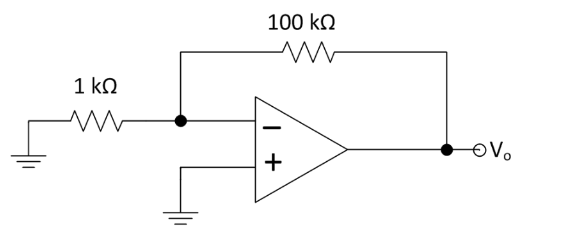
\includegraphics[width=0.6\textwidth]{15.png} 
      \caption{}
    \label{fig:fig15} 
\end{figure}
\hfill(GATE IN 2023)

    \item The force per unit length between two infinitely long parallel conductors, with a gap of 2 cm between them is 10 $\mu$N/m. When the gap is doubled, the force per unit length will be \_\_\_\_\_ $\mu$N/m (rounded off to one decimal place).
\hfill(GATE IN 2023)

    \item Consider the discrete-time signal $x[n] = u[-n + 5] - u[n + 3]$, where $u[n] = \begin{cases} 1 & n \geq 0 \\ 0 & n < 0 \end{cases}$. The smallest $n$ for which $x[n] = 0$ is \_\_\_\_\_.
\hfill(GATE IN 2023)

    \item Let $y(t) = x(4t)$, where $x(t)$ is a continuous-time periodic signal with fundamental period of 100 s. The fundamental period of $y(t)$ is \_\_\_\_\_ s (rounded off to the nearest integer).
\hfill(GATE IN 2023)

    \item When the bridge given below is balanced, the current through the resistor $R_a$ is \_\_\_\_\_ mA (rounded off to two decimal places).
    \begin{figure}[H]
    \centering
      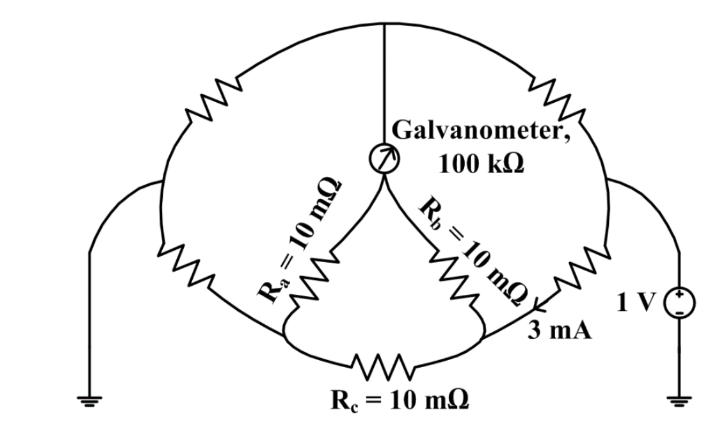
\includegraphics[width=0.6\textwidth]{16.png} 
      \caption{}
    \label{fig:fig16} 
\end{figure}
\hfill(GATE IN 2023)

    \item In the circuit given, the Thevenin equivalent resistance $R_{th}$ across the terminals 'a' and 'b' is \_\_\_\_\_ $\Omega$ (rounded off to one decimal place).
    \begin{figure}[H]
    \centering
      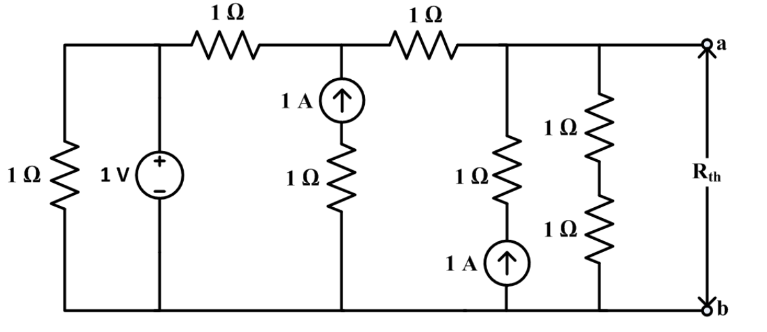
\includegraphics[width=0.6\textwidth]{17.png} 
      \caption{}
    \label{fig:fig17} 
\end{figure}
\hfill(GATE IN 2023)

    \item $X$ is a discrete random variable which takes values 0, 1 and 2. The probabilities are $P(X = 0) = 0.25$ and $P(X = 1) = 0.5$. With $E[\cdot]$ denoting the expectation operator, the value of $E[X] - E[X^2]$ is \_\_\_\_\_ (rounded off to one decimal place).
\hfill(GATE IN 2023)

    \item The diode in the circuit is ideal. The current source $i_s(t) = \pi \sin (3000\pi t)$ mA. The magnitude of the average current flowing through the resistor $R$ is \_\_\_\_\_ mA (rounded off to two decimal places).
    \begin{figure}[H]
    \centering
      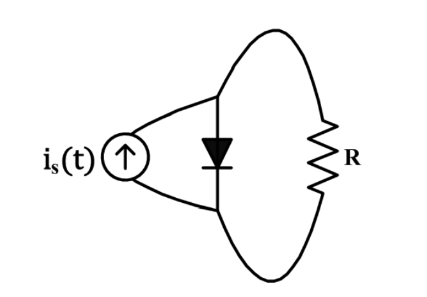
\includegraphics[width=0.6\textwidth]{18.png} 
      \caption{}
    \label{fig:fig18} 
\end{figure}
\hfill(GATE IN 2023)

    \item The full-scale range of the wattmeter shown in the circuit is 100 W. The turns ratio of the individual transformers are indicated in the figure. The RMS value of the ac source voltage $V_s$ is 200 V. The wattmeter reading will be \_\_\_\_\_ W (rounded off to the nearest integer).
    \begin{figure}[H]
    \centering
      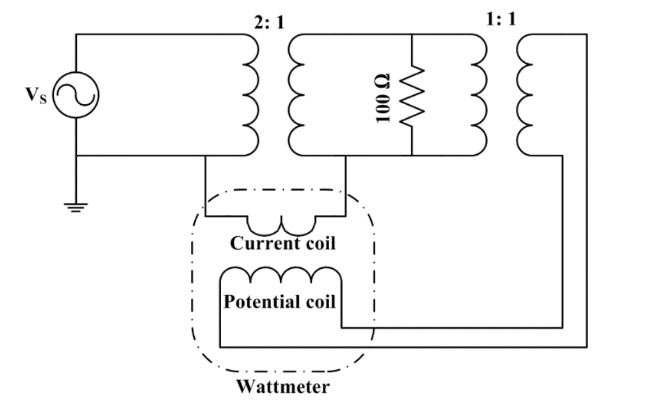
\includegraphics[width=0.6\textwidth]{19.png} 
      \caption{}
    \label{fig:fig19} 
\end{figure}
\hfill(GATE IN 2023)

    \item The no-load steady-state output voltage of a DC shunt generator is 200 V when it is driven in the clockwise direction at its rated speed. If the same machine is driven at the rated speed but in the opposite direction, the steady-state output voltage will be \_\_\_\_\_ V (rounded off to the nearest integer).
\hfill(GATE IN 2023)

    \item The impulse response of an LTI system is $h(t) = \delta(t) + 0.5 \delta(t-4)$, where $\delta(t)$ is the continuous-time unit impulse signal. If the input signal $x(t) = \cos\left(\frac{7\pi t}{4}\right)$, the output is \_\_\_\_\_.
    
    \begin{enumerate}
        \item $0.5 \cos\left(\frac{7\pi t}{4}\right)$
        \item $1.5 \cos\left(\frac{7\pi t}{4}\right)$
        \item $0.5 \sin\left(\frac{7\pi t}{4}\right)$
        \item $1.5 \sin\left(\frac{7\pi t}{4}\right)$
    \end{enumerate}
    \hfill(GATE IN 2023)

    \item The Laplace transform of the continuous-time signal $x(t) = e^{-3t} u(t-5)$ is \_\_\_\_\_, where $u(t)$ denotes the continuous-time unit step signal.
    
    \begin{enumerate}
        \item $\frac{e^{-5s}}{s+3}$, Real[$s$] $> -3$
        \item $\frac{e^{-5(s-3)}}{s-3}$, Real[$s$] $> 3$
        \item $\frac{e^{-5(s+3)}}{s+3}$, Real[$s$] $> -3$
        \item $\frac{e^{-5(s-3)}}{s+3}$, Real[$s$] $> -3$
    \end{enumerate}
    \hfill(GATE IN 2023)

    \item In a p-i-n photodiode, a pulse of light containing $8 \times 10^{12}$ incident photons at wavelength $\lambda_0 = 1.55$ $\mu$m gives rise to an average $4 \times 10^{12}$ electrons collected at the terminals of the device. The quantum efficiency of the photodiode at this wavelength is \_\_\_\_\_ \%.
    
    \begin{enumerate}
        \item 50
        \item 54.2
        \item 62.5
        \item 80
    \end{enumerate}
    \hfill(GATE IN 2023)

    \item Let $f(z) = j \frac{1-z}{1+z}$, where $z$ denotes a complex number and $j$ denotes $\sqrt{-1}$. The inverse function $f^{-1}(z)$ maps the real axis to the \_\_\_\_\_.
    
    \begin{enumerate}
        \item unit circle with centre at the origin
        \item unit circle with centre not at the origin
        \item imaginary axis
        \item real axis
    \end{enumerate}
    \hfill(GATE IN 2023)

    \item The simplified form of the Boolean function $F(W, X, Y, Z) = \sum (4, 5, 10, 11, 12, 13, 14, 15)$ with the minimum number of terms and smallest number of literals in each term is\_\_\_\_\_.
    
    \begin{enumerate}
        \item $WX + \overline{W}X\overline{Y} + W\overline{X}Y$
        \item $WX + WY + X\overline{Y}$
        \item $X\overline{Y} + WY$
        \item $\overline{X}Y + \overline{WY}$
    \end{enumerate}
    \hfill(GATE IN 2023)

    \item For the given digital circuit, $A = B = 1$. Assume that AND, OR, and NOT gates have propagation delays of 10 ns, 10 ns, and 5 ns respectively. All lines have zero propagation delay. Given that $C = 1$ when the circuit is turned on, the frequency of steady-state oscillation of the output $Y$ is \_\_\_\_\_.
    \begin{figure}[H]
    \centering
      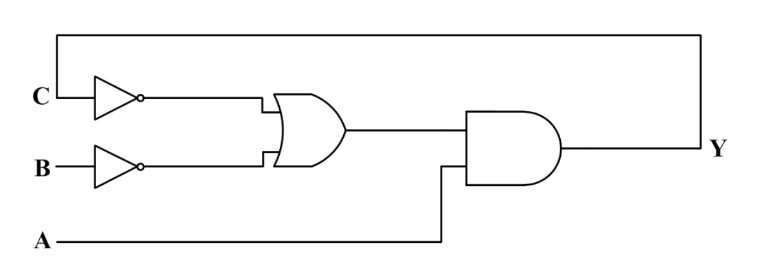
\includegraphics[width=0.6\textwidth]{20.png} 
      \caption{}
    \label{fig:fig20} 
\end{figure}
    \begin{enumerate}
        \item 20 MHz
        \item 15 MHz
        \item 40 MHz
        \item 50 MHz
    \end{enumerate}
    \hfill(GATE IN 2023)

    \item In the circuit shown, the initial binary content of shift register A is 1101 and that of shift register B is 1010. The shift registers are positive-edge triggered, and the gates have no delay. When the shift control is high, what will be the binary content of the shift registers A and B after four clock pulses?
    \begin{figure}[H]
    \centering
      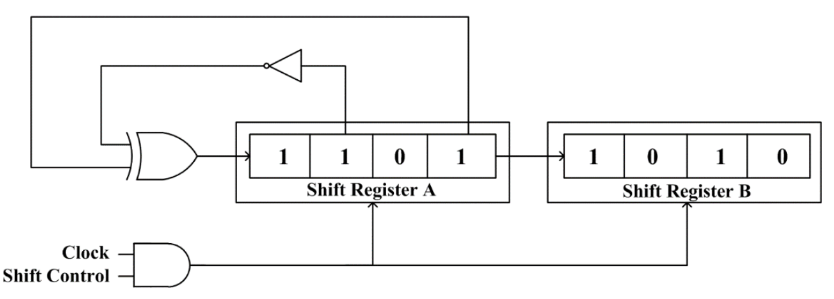
\includegraphics[width=0.6\textwidth]{21.png} 
      \caption{}
    \label{fig:fig21} 
\end{figure}
    \begin{enumerate}
        \item A = 1101, B = 1101
        \item A = 1110, B = 1001
        \item A = 0101, B = 1101
        \item A = 1010, B = 1111
    \end{enumerate}
    \hfill(GATE IN 2023)

    \item The magnitude and phase plots shown in the figure match with the transfer-function\_\_\_\_\_.
    \begin{figure}[H]
    \centering
      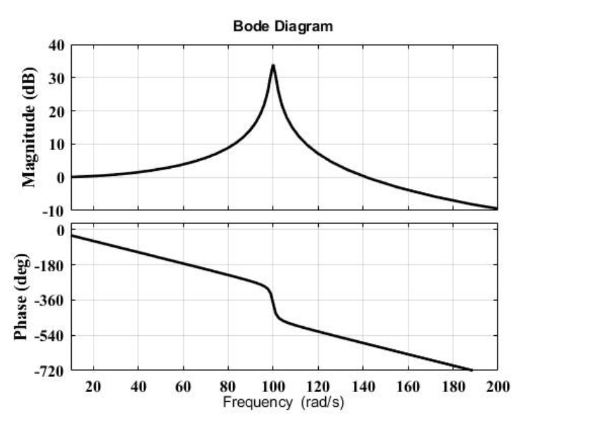
\includegraphics[width=0.6\textwidth]{22.png} 
      \caption{}
    \label{fig:fig22} 
\end{figure}
    \begin{enumerate}
        \item $\frac{10000}{s^2 + 2s + 10000}$
        \item $\frac{10000 e^{-0.05s}}{s^2 + 2s + 10000}$
        \item $\frac{10000 e^{-0.5 \times 10^{-12}s}}{s^2 + 2s + 10000}$
        \item $\frac{100}{s^2 + 2s + 100}$
    \end{enumerate}
    \hfill(GATE IN 2023)

    \item A continuous real-valued signal $x(t)$ has finite positive energy and $x(t) = 0$, $\forall t < 0$. From the list given below, select ALL the signals whose continuous-time Fourier transform is purely imaginary.
    
    \begin{enumerate}
        \item $x(t) + x(-t)$
        \item $x(t) - x(-t)$
        \item $j(x(t) + x(-t))$
        \item $j(x(t) - x(-t))$
    \end{enumerate}
    \hfill(GATE IN 2023)

    \item A silica-glass fiber has a core refractive index of 1.47 and a cladding refractive index of 1.44. If the cladding is completely stripped out and the core is dipped in water having a refractive index of 1.33, the numerical aperture of the modified fiber is\_\_\_\_\_ (rounded off to three decimal places).
\hfill(GATE IN 2023)
    \item In the circuit shown, $\omega = 100\pi$ rad/s, $R_1 = R_2 = 2.2$ $\Omega$ and $L = 7$ mH. The capacitance $C$ for which $Y_{in}$ is purely real is \_\_\_\_\_ mF (rounded off to two decimal places).
    \begin{figure}[H]
    \centering
      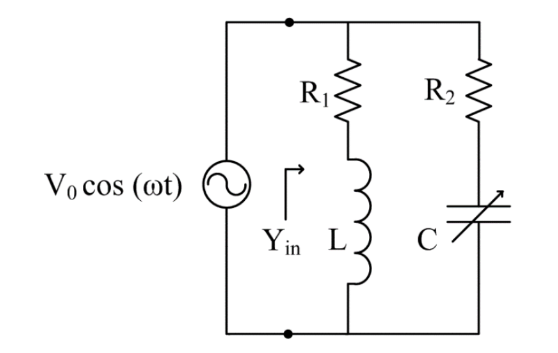
\includegraphics[width=0.6\textwidth]{23.png} 
      \caption{}
    \label{fig:fig23} 
\end{figure}
\hfill(GATE IN 2023)
    \item The R-L circuit with $R = 10$ k$\Omega$ and $L = 1$ mH is excited by a step current $I_0 u(t)$. At $t = 0^-$, there is a current $I_L = I_0/5$ flowing through the inductor. The minimum time taken for the current through the inductor to reach 99\% of its final value is \_\_\_\_\_ $\mu$s (rounded off to two decimal places).
    \begin{figure}[H]
    \centering
      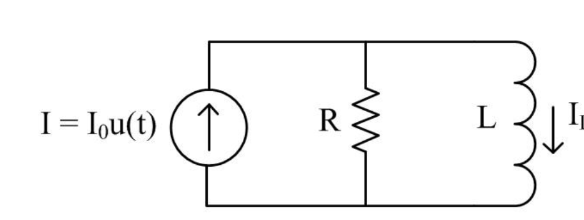
\includegraphics[width=0.6\textwidth]{24.png} 
      \caption{}
    \label{fig:fig24} 
\end{figure}
\hfill(GATE IN 2023)
    \item Consider a standard negative feedback configuration with $G(s) = \frac{1}{(s-2)(s-3)}$ and the controller $C(s) = K_p + \frac{K_I}{s} + K_D s$. The root-locus of $G(s)C(s)$ is presented in the figure below. The gain $C(j\omega) = 2$ at $\omega = 1$ rad/s. The value of $K_D$ is \_\_\_\_\_ (rounded off to one decimal place).
    \begin{figure}[H]
    \centering
      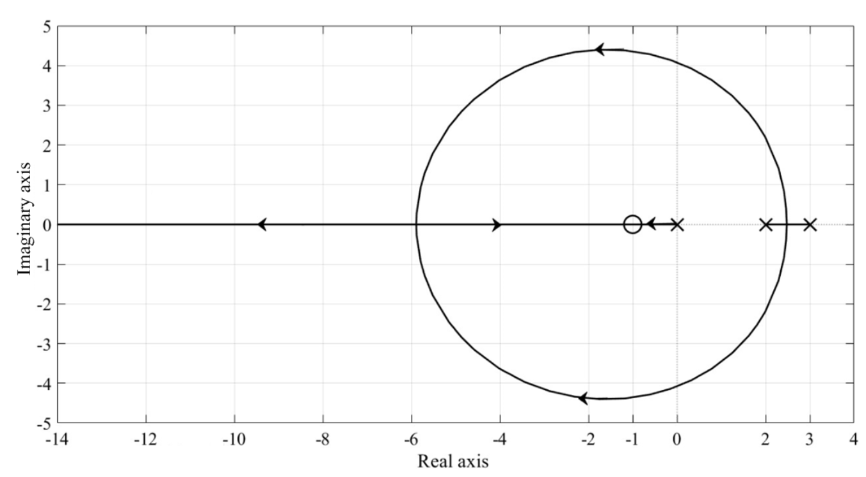
\includegraphics[width=0.6\textwidth]{25.png} 
      \caption{}
    \label{fig:fig25} 
\end{figure}
\hfill(GATE IN 2023)
    \item How many five-digit numbers can be formed using the integers 3, 4, 5 and 6 with exactly one digit appearing twice?
\hfill(GATE IN 2023)
    \item The phase margin of the transfer function $G(s) = \frac{2(1-s)}{(1+s)^2}$ is \_\_\_\_\_ degrees (rounded off to the nearest integer).
\hfill(GATE IN 2023)
    \item A wire-wound 'resistive potentiometer type' angle sensor with 72 turns is used in an application. The first turn of the potentiometer is connected to ground while its last turn is connected to 3.6 V. The width of the wiper covers two turns ensuring make-before-break. The output (wiper) voltage when the wiper is on top of both the turns 35 and 36 is \_\_\_\_\_ V (rounded off to two decimal places).
\hfill(GATE IN 2023)
    \item The two secondaries of a linear variable differential transformer (LVDT) showed a magnitude of 2 V (RMS) for zero displacement position of the core. It is noted that the phase of one of the secondaries has a deviation of one degree from the expected phase. Other than this deviation, the LVDT is ideal. If the differential output sensitivity of the LVDT is 1 mV (RMS)/1 $\mu$m, the output for zero displacement is \_\_\_\_\_ $\mu$m (rounded off to one decimal place).
\hfill(GATE IN 2023)
    \item Five measurements are made using a weighing machine, and the readings are 80 kg, 79 kg, 81 kg, 79 kg and 81 kg. The sample standard deviation of the measurement is \_\_\_\_\_ kg (rounded off to two decimal places).
\hfill(GATE IN 2023)
    \item Four strain gauges $R_A$, $R_B$, $R_C$ and $R_D$, each with nominal resistance $R$, are connected in a bridge configuration. When a force is applied, $R_A$ and $R_D$ increase by $\Delta R$ and $R_B$ and $R_C$ decrease by $\Delta R$ as shown. A potentiometer with total resistance $R_v$ is connected as shown. If $R = 100$ $\Omega$, and $\Delta R = 1$ $\Omega$, the minimum value of resistance $R_v$ required to balance the bridge is \_\_\_\_\_ $\Omega$ (rounded off to two decimal places).
    \begin{figure}[H]
    \centering
      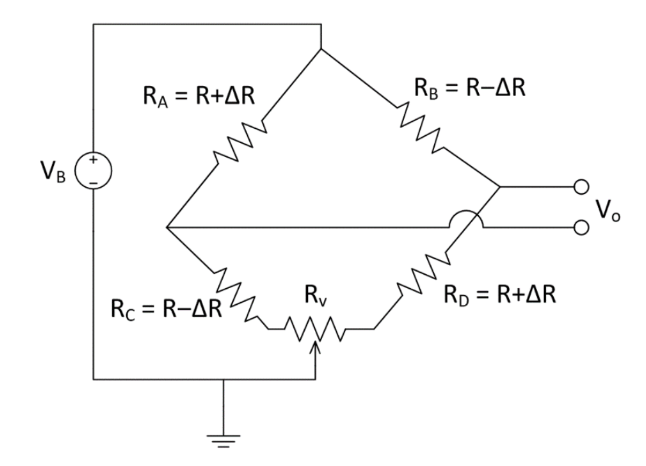
\includegraphics[width=0.6\textwidth]{26.png} 
      \caption{}
    \label{fig:fig26} 
\end{figure}
\hfill(GATE IN 2023)
    \item A sinusoidal current of $i_1(t) = 1 \sin(200\pi t)$ mA is flowing through a 4 H inductor which is mutually coupled to another 5 H inductor carrying $i_2(t) = 2 \sin(200\pi t)$ mA as shown in the figure. The coupling coefficient between the inductors is 0.6. The peak energy stored in the circuit is \_\_\_\_\_ $\mu$J (rounded off to two decimal places).
    \begin{figure}[H]
    \centering
      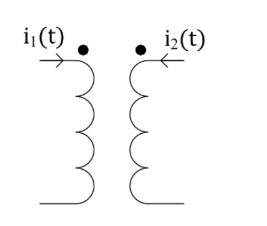
\includegraphics[width=0.6\textwidth]{27.png} 
      \caption{}
    \label{fig:fig27} 
\end{figure}
\hfill(GATE IN 2023)
    \item The figure below shows a feedback amplifier constructed using an nMOS transistor. Assume that $\mu_n C_{ox} = 1$ mA/V$^2$, threshold voltage $V_T = 1$ V and $W/L = 2$. The bias voltage at the drain terminal is 4 V. The capacitors $C_{\infty}$ offer zero impedance at the signal frequency. The ratio $V_{out}/V_{in}$ is \_\_\_\_\_ (rounded off to two decimal places).
    \begin{figure}[H]
    \centering
      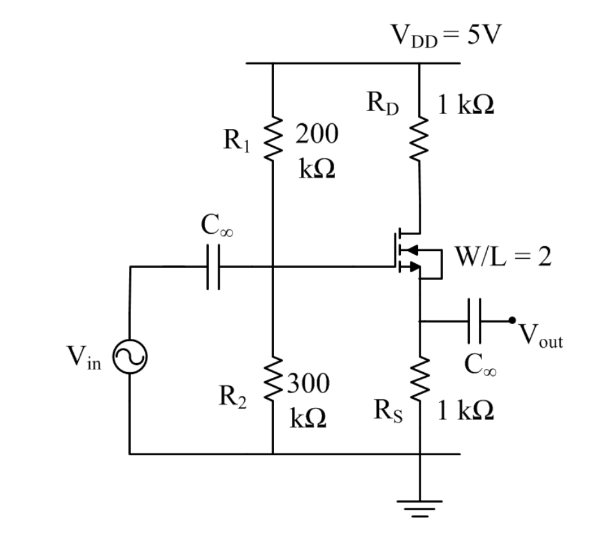
\includegraphics[width=0.6\textwidth]{28.png} 
      \caption{}
    \label{fig:fig28} 
\end{figure}
\hfill(GATE IN 2023)
    \item Consider the real-valued function $g(x) = \max[(x-2)^2, -2x + 7]$, where $x \in (-\infty, \infty)$. The minimum value attained by $g(x)$ is \_\_\_\_\_ (rounded off to one decimal place).
\hfill(GATE IN 2023)
    \item A short-circuit test is conducted on a single-phase transformer by shorting its secondary. The frequency of input voltage is 1 kHz. The corresponding wattmeter reading, primary current and primary voltage are 8 W, 2 A and 6 V respectively. Assume that the no-load losses and the no-load currents are negligible, and the core has linear magnetic characteristics. Keeping the secondary shorted, the primary is connected to a 2 V (RMS), 1 kHz sinusoidal source in series with a $\frac{1}{2\pi\sqrt{5}}$ mF capacitor. The primary current (RMS) will be \_\_\_\_\_ A (rounded off to two decimal places).
\hfill(GATE IN 2023)
    \item The opamps in the circuit are ideal. The input signals are $V_{s1} = 3 + 0.10 \sin(300t)$ V and $V_{s2} = -2 + 0.11 \sin(300t)$ V. The average value of the voltage $V_0$ is \_\_\_\_\_ V (rounded off to two decimal places).
    \begin{figure}[H]
    \centering
      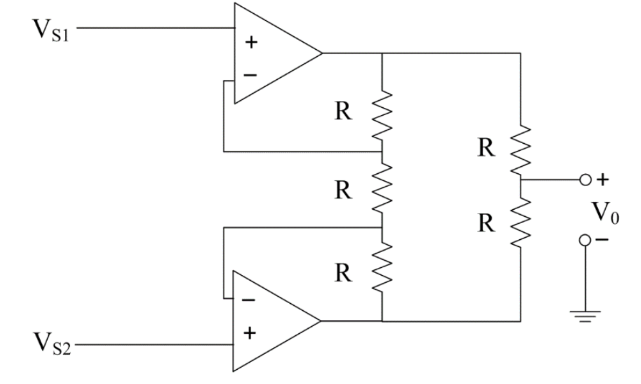
\includegraphics[width=0.6\textwidth]{29.png} 
      \caption{}
    \label{fig:fig29} 
\end{figure}
\hfill(GATE IN 2023)
    \item In the circuit shown, the input voltage $V_{in} = 100$ mV. The switch and the opamp are ideal. At time $t = 0$, the initial charge stored in the 10 nF capacitor is 1 nC, with the polarity as indicated in the figure. The switch S is controlled using a 1 kHz square-wave voltage signal $V_s$ as shown. Whenever $V_s$ is 'High', S is in position '1' and when $V_s$ is 'Low', S is in position '2'. At $t = 20$ ms, the magnitude of the voltage $V_o$ will be \_\_\_\_\_ mV (rounded off to the nearest integer).
    \begin{figure}[H]
    \centering
      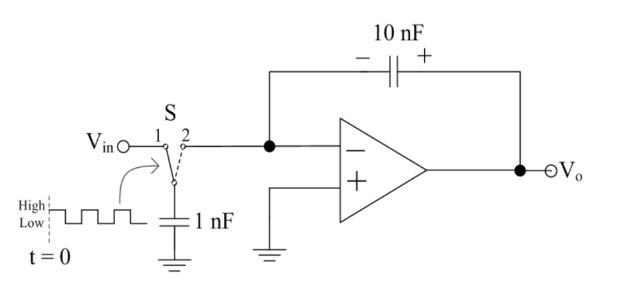
\includegraphics[width=0.6\textwidth]{30.png} 
      \caption{}
    \label{fig:fig30} 
\end{figure}
\hfill(GATE IN 2023)
    \item In the diagram shown, the frequency of the sinusoidal source voltage $V_S$ is 50 Hz. The load voltage is 230 V (RMS), and the load impedance is $\frac{230}{\sqrt{2}} + j\frac{230}{\sqrt{2}}$ $\Omega$. The value of attenuator $A_1 = \frac{1}{50\sqrt{2}}$. The multiplier output voltage $V_o = \frac{V_x V_y}{1 V}$, where $V_x$ and $V_y$ are the inputs. The magnitude of the average value of the multiplier output $V_o$ is \_\_\_\_\_ V (rounded off to one decimal place).
    \begin{figure}[H]
    \centering
      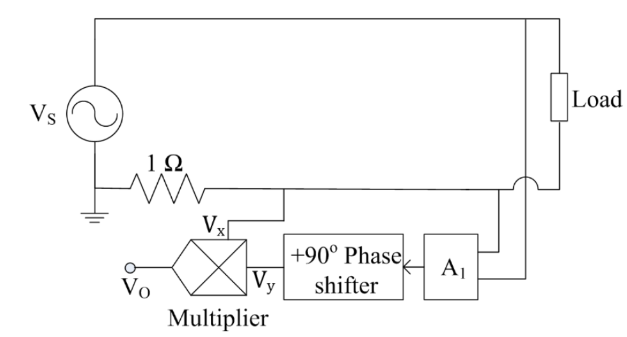
\includegraphics[width=0.6\textwidth]{31.png} 
      \caption{}
    \label{fig:fig31} 
\end{figure}
\hfill(GATE IN 2023)
    \item In the circuit shown, assuming an ideal opamp, the value of the output voltage $V_0 =$ \_\_\_\_\_ V (rounded off to one decimal place).
    \begin{figure}[H]
    \centering
      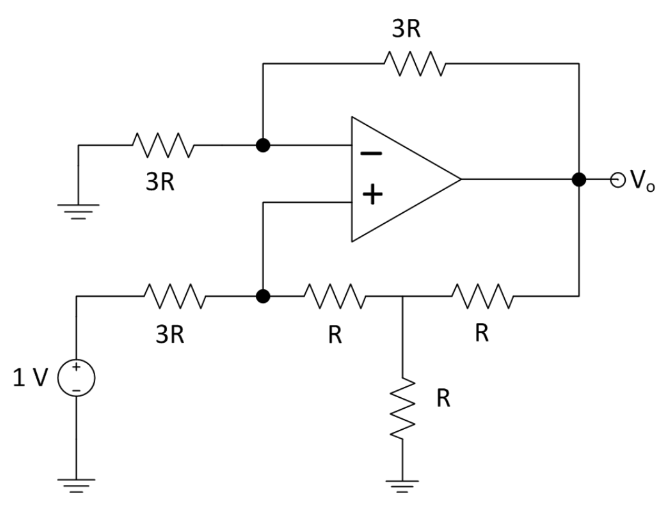
\includegraphics[width=0.6\textwidth]{32.png} 
      \caption{}
    \label{fig:fig32} 
\end{figure}
\hfill(GATE IN 2023)
    \item The rank of the matrix $A$ given below is one. The ratio $\frac{\alpha}{\beta}$ is \_\_\_\_\_ (rounded off to the nearest integer).
    $\Vec{A} = \myvec{ 1 & 4 \\ -3 & \alpha \\ \beta & 6 }$
\hfill(GATE IN 2023)
    \item A 1.999 V True RMS 3-1/2 digit multimeter has an accuracy of $\pm 0.1\%$ of reading $\pm 2$ digits. It is used to measure 100 A (RMS) current flowing through a line using a 100:5 ratio, Class-1 current transformer with a burden of 0.1 $\Omega$ $\pm 0.5\%$. The worst-case absolute error in the multimeter output is \_\_\_\_\_ V (rounded off to three decimal places).
\hfill(GATE IN 2023)
    \item The voltage source $V_s = 10\sqrt{2} \sin(20000\pi t)$ V has an internal resistance of 50 $\Omega$. The RMS value of the current through $R$ is\_\_\_\_\_ mA (rounded off to one decimal place).
    \begin{figure}[H]
    \centering
      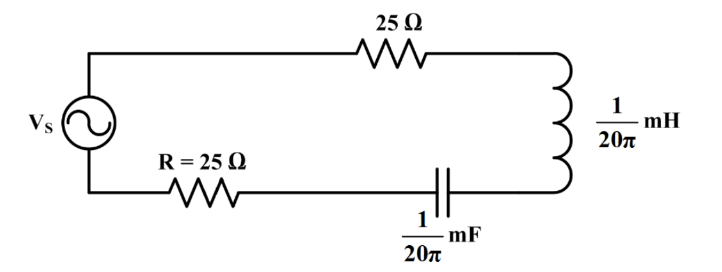
\includegraphics[width=0.6\textwidth]{33.png} 
      \caption{}
    \label{fig:fig33} 
\end{figure}
\hfill(GATE IN 2023)
\end{enumerate}

\end{document}
